We start by developing a simple theoretical setup that relates polarization to mobility. We consider three types of jobs $j = \{1,2,3\}$, which can be interpreted, respectively, as low-paying, middling and high-paying jobs. Parents transfer human capital to their children and the latter’s productivity, and hence allocation to jobs, is determined both by transmitted human capital and innate (and initially unobservable) ability. Children’s entry jobs will be determined by parental background, but as their ability is revealed, they may move up or down the job ladder. The aim of the model is to illustrate how mobility changes as the share of middling jobs falls.

\subsection{Workers' skills and family background} \label{chap2-model-workers}

We suppose that there are two types of parental background, which we denote by low-income ($L$) and high-income ($H$). The difference between the two groups can encompass income or human capital; what is important for our purposes is that children of $H$-parents have more initial human capital than those of $L$-parents, whether through direct transmission or the possibility of accessing better schools or more years of education. We denote by $z_i$ the share of parents with background $i = \{L,H\}$, with $z_H + z_L = 1$.

Individuals also differ in their innate ability, which will be high with probability $\pi$ and low otherwise, and is assumed not to depend on parental type. Ability is assumed to have no effect on first-period productivity but will affect that in the second period. Ability is potentially observable---by the individual and by the firm---at the end of the first period. We suppose that the individual can always observe her ability but has no way of truthfully revealing it to the firm. Our key assumption is that whether ability is observed by the firm depends on the type of job that the individual performed in the first period. In particular, we suppose that ability is observed by the firm if the individual worked in middling or high-paying occupations but not if she worked in a low-paying occupation. \footnote{The underlying idea is that the simple tasks performed in this kind of occupation make it impossible to infer how capable the individual will be in other types of occupations. Alternatively, we could have considered the possibility that certain jobs allow for the accumulation of human capital which is complementary with ability, while others do not.} 

Assuming that parental type perfectly determines the initial skills of the child, the human capital of an individual in the first period is simply $h_L$ or $h_H$ for those with low- and high-income parents, respectively, and there will be a share $z_L$  and $z_H$ of young individuals of each type. Second period productivity is supposed to depend on both parental background and ability. We denote by $\underline{h}_i$, respectively $\overline{h}_i$, the second-period human capital of an individual of type $i$ that is of low, respectively high, ability. The resulting productivities are ranked as follows: $\underline{h}_L < \underline{h}_H < \overline{h}_L < \overline{h}_H$, implying that while parental background matters, high ability individuals are always more productive than those with low ability irrespective of family background. 

\subsection{The structure of employment} \label{chap2-model-structure}

Denote the share of low-paying jobs by $q_1$, the share of middling jobs by $q_2$, and the share of high-paying jobs by $q_3$. . Since the wage of high-paying (resp. middling) jobs is greater than that of middling (resp. low-paying) jobs, employers fill jobs of each type with the most skilled worker available. 
The model can present various allocations of individuals across occupations depending on parameter values. We focus in a particular case which illustrates the mechanism we have in mind. To do so we make two assumption on parameter values:
\begin{assumption}\label{chap2-ass:threshold-skill-p1}
We suppose that the share of low-income parents, $z_L$, satisfies $1-q_3 > z_L > q_1$.
\end{assumption}
Assumption \ref{chap2-ass:threshold-skill-p1} ensures that in the first period some individuals from both high- and low-income parental backgrounds are in occupation 2.
\begin{assumption}\label{chap2-ass:threshold-skill-p2}
We suppose that the share of high-ability individuals, $\pi$, satisfies $ \frac{q_3}{1-q_1} > \pi > 1- \frac{q_1}{z_L-q_1} $.
\end{assumption}
Assumption \ref{chap2-ass:threshold-skill-p2} characterizes the second period allocations. It ensures that (i) not all low-ability individuals from low-income households work in occupation 1 and (ii) some low-ability individuals from high-income household work in occupation 3. 

\subsection{The allocation of labour} \label{chap2-model-allocation}

Employers fill jobs sequentially according to the worker's human capital. Table \ref{chap2-tab:init-prb-p1} summarizes, under Assumption \ref{chap2-ass:threshold-skill-p1}, the distributions of jobs in the first period. The distribution of jobs and skills in the population are such that only workers with low-income (resp. high-income) parents are initially in low-paid (resp. high-paid) occupations, while both types of individuals are found in middling jobs in the first period.

\begin{table}[!htb]
    \centering
    \caption{First-period allocation of labour}
    \label{chap2-tab:init-prb-p1}
    \begin{threeparttable}
        \setlength{\tabcolsep}{12pt}
        \setlength{\extrarowheight}{6pt}
        \begin{tabular}{r|c|c}
            & $L$ & $H$ \\
            \midrule
            Low-paying & $q_1$ & $0$ \\
            Middling & $z_L - q_1$ & $z_H - q_3$ \\
            High-paying & $0$ & $q_3$
        \end{tabular}
    \end{threeparttable}
\end{table}

In the second period, the allocation of individuals across jobs depends on three factors: parental background, ability, and the occupation in which the individual worked in the first period. Notably, the latter matters because of our assumption that ability is not revealed for those in low-paying occupations. 

Consider those who start in low-paying occupations and for whom ability is not revealed. Firms will attribute them their expected productivity which is given by $\widehat{h}_L\equiv (1-\pi )\underline{h}_{L}+\pi \overline{h}_{L}$. We assume this expression to satisfy $ \underline{h}_{L} < \widehat{h}_L < \underline{h}_{H} $. That is, those who have worked in low-paying occupations have an expected skill level above the low-ability $L$-parent workers that worked in middling occupations but below that of low-ability $H$-parent individuals. The distribution of expected skills is then
\begin{equation*}
    h=\left\{ 
        \begin{array}{cc}
            \underline{h}_{L} & (1-\pi )(z_{L}-q_1) \\ 
            \widehat{h}_L & q_{1} \\ 
            \underline{h}_{H} & (1-\pi )z_{H} \\ 
            \overline{h}_{L} & \pi (z_{L}-q_1) \\ 
            \overline{h}_{H} & \pi z_{H}
        \end{array}
    \right.  
\end{equation*}

We can now consider the allocation of workers to occupations in the second period. Under Assumptions \ref{chap2-ass:threshold-skill-p1} and \ref{chap2-ass:threshold-skill-p2}, low-paying jobs are filled with individuals from low-income households, while middling and high-paying jobs contain workers from both low- and high-income households (see Appendix \ref{chap2-app-model} for the details). Let $P_i(k)$ be the probability that an individual of background $i$ is in occupation $k$ in the second period. 
Table \ref{chap2-tab:uncond-prb-p2} summarizes these probabilities.
\begin{table}[!htb]
    \centering
    \caption{Second-period allocation of labour}
    \label{chap2-tab:uncond-prb-p2}
    \begin{threeparttable}
        \setlength{\tabcolsep}{12pt}
        \setlength{\extrarowheight}{6pt}
        \begin{tabular}{r|c|c}
                        & $L$ & $H$ \\
            \midrule
            Low-paying  & $\frac{q_{1}}{z_{L}}$ & $0$ \\
            Middling    & $(1-\pi)\left(1-\frac{q_1}{z_L}\right) $ & $1- \pi - \frac{q_{3}-\pi (1-q_{1})}{z_{H}}$ \\
            High-paying & $\pi \left(1-\frac{q_1}{z_L}\right)$ & $\pi +\frac{q_{3}-\pi (1-q_{1})}{z_{H}}$
        \end{tabular}
    \end{threeparttable}
\end{table}

Changes in $q_{1}$ and $q_{3}$ have both direct and indirect effects. The direct effects stem from the fact that there are more or fewer jobs of type $k$ available; the indirect ones are due to the information friction that prevents the ability of certain workers from being revealed. Consider, for example, the occupational outcomes of individuals with low-income parents. A higher value of $q_1$ increases the likelihood that they work in low-paying occupations simply because there are more of these positions, which would tend to increase the share of $L$-workers in low-paying occupations and decrease that in middling occupations. Yet the share of $L$-workers in high-paying occupations also falls in response  to a higher value of $q_{1}$ due to the indirect effect stemming from the different information content of the various jobs. A higher value of $q_{1}$ implies that in the first period fewer $L$-workers were in occupation 2 and hence fewer of them revealed that they are high ability, thus reducing the share of $L$-workers that manage to move to high-paying occupations.

The second-period allocation of workers from high-income families depends on both $q_{1}$ and $q_{3}$. A higher share of high-paying jobs, $q_{3}$, will tend to increase the probability of working in type-3 occupations by allowing some low-ability individuals from wealthy households to have access to those jobs. But the extent to which this happens depends on $q_{1}$. A higher value of $q_{1}$ implies that fewer $L$-worker have revealed to be of high-ability and hence fewer of them will have moved from occupation 2 to occupation 3. More high-paying jobs are hence available to be filled by low-ability $H$-workers. These results indicate that the information content of middling jobs plays a key role in shaping the allocation of employment of mature workers. In Appendix \ref{chap2-app-model} we examine in detail the extent to which this results are driven by the direct effect of job availability or by the information friction. What is interesting for our purposes is that while the direct effect does not allow for an improvement in the allocation of workers to jobs, the effect of the information friction does. The friction implies that there are individuals in high-paying whose productivity is lower than that of others that are in low-paying or middling occupations.


\subsection{Transition probabilities}

Table \ref{chap2-tab:uncond-prb-p2} captures the extent of inter-generational mobility, which in turn depends both on the effect of parental background on entry positions and on the probabilities of moving across occupations between periods 1 and 2. The latter, which we can think of as intra-generational mobility, can be computed as the probability $P_i(k|j)$ that an individual of parental background $i$ and initial occupation $j$ ends in occupation $k$ when mature. Table \ref{chap2-tab:trans-prb} summarizes the transition probabilities.  
\begin{table}[!htb]
    \setlength{\tabcolsep}{6pt}
    \setlength{\extrarowheight}{8pt}
    \caption{Transition probabilities across occupations}\label{chap2-tab:trans-prb}
    \centering
    \begin{tabular}{rcccc}
    \toprule
        & & End 1 & End 2 & End 3\\\midrule
         \multirow{2}{*}{L-workers} & Initial 1 & $1-(1-\pi)\frac{z_{L}-q_1}{q_1}$ & $(1-\pi )\frac{z_{L}-q_1}{q_{1}}$ & 0 \\
         & Initial 2 & $1-\pi$ & 0 & $\pi$ \\
         \midrule
         \multirow{2}{*}{H-workers} & Initial 2 & 0 & $1-\pi$ & $\pi$\\
         & Initial 3 & 0 & $1 - \pi - \frac{q_3 - \pi (1-q_{1}) }{q_{3}}$ & $\pi + \frac{q_3 - \pi (1-q_{1}) }{q_{3}}$\\
         \bottomrule
    \end{tabular}
\end{table}

Recall that those from an $L$-background are randomly allocated across occupations 1 and 2 in the first period. Those who start in 2 will either move upwards or downwards depending on their revealed ability but independently of the distribution of occupations. The outcome for those who start their careers in 1 depends on $q_1$, with a higher share of low-paying jobs leading to lower upwards mobility (i.e. into middling occupations) for this group. 

Consider now $H$-workers and note that, by Assumption \ref{chap2-ass:threshold-skill-p2}, $q_3 - \pi (1-q_{1})>0$. For those who started in middling occupation, whether or not they move into high-paying occupations depends exclusively on their ability, so that they have a probability $\pi$ (resp. $1-\pi$) or being in occupation 3 (resp. 2) in the second period. For those who started in occupation 3, the likelihood of downwards mobility depends on both $q_1$ and $q_3$, with higher values of either resulting in a lower probability that (low-ability) $H$-workers move downwards.

\subsection{The impact of polarization} \label{chap2-model-polarization}

We can now consider how polarization affects inter-generational mobility. We define \textit{polarization} as a simultaneous increase in $q_{1}$ and $q_{3}$ at the expense of $q_{2}$. For ease of exposition, we suppose that the share of the two occupations increases by the same amount and that there is no change between the two periods of an individual's active life.\footnote{Other scenarii are possible and would make the model richer, notably by allowing for different degrees of polarization when individuals are young and when they are mature.}

Polarization affects both entry jobs and the transition probabilities (intra-generational mobility), which together will shape the extent of inter-generational mobility. We consider the impact on each in turns, recalling, as discussed above, that changes in the structure of employment have both a direct and an indirect effect. Greater polarization has only the direct effect on the first-period allocation of labour, and, as can be seen in Table \ref{chap2-tab:init-prb-p1}, it increases in a mechanical way the share of individuals with low-income (resp. high-income) parents that are in low-paying (resp. high-paying) occupations. That is, greater polarization implies a stronger influence of parental income on the occupations of young agents. 

The transition probabilities across occupations are affected by both the availability of jobs when individuals are mature and by the fact that the number of $L$-background individuals who were in middling occupations determines how many of them will experience upwards mobility. As can be seen from Table \ref{chap2-tab:trans-prb}, an increase in $q_1$, $q_3$, or both reduces the likelihood to escape the initial occupation, thus causing more intra-generational persistence. 

Since in our framework first-period occupations depend only on parental income, higher intra-generational persistence undermines inter-generational mobility. To see this, we turn now to the probabilities of being in the various occupations when mature as given by Table \ref{chap2-tab:uncond-prb-p2}. There are various ways of measuring inter-generational mobility. To capture it in a simple way, we measure it by the advantage that parental background gives in terms of accessing the various occupations. We hence define \textit{inter-generational mobility} as the gap between $H$-workers and $L$-workers in the probability of being in each occupation, that is, $\Delta P(k) = P_H(k)-P_L(k)$, where the relevant probabilities are given in Table \ref{chap2-tab:uncond-prb-p2}.

Figure \ref{chap2-fig:theory-proba-gap} presents the relationship between mobility and polarization.
\begin{figure}[!tb]
    \centering
    \caption{Probability gap in second-period occupations between $H$ and $L$ background according to change in $q_1$ and $q_3$}
    \label{chap2-fig:theory-proba-gap}
    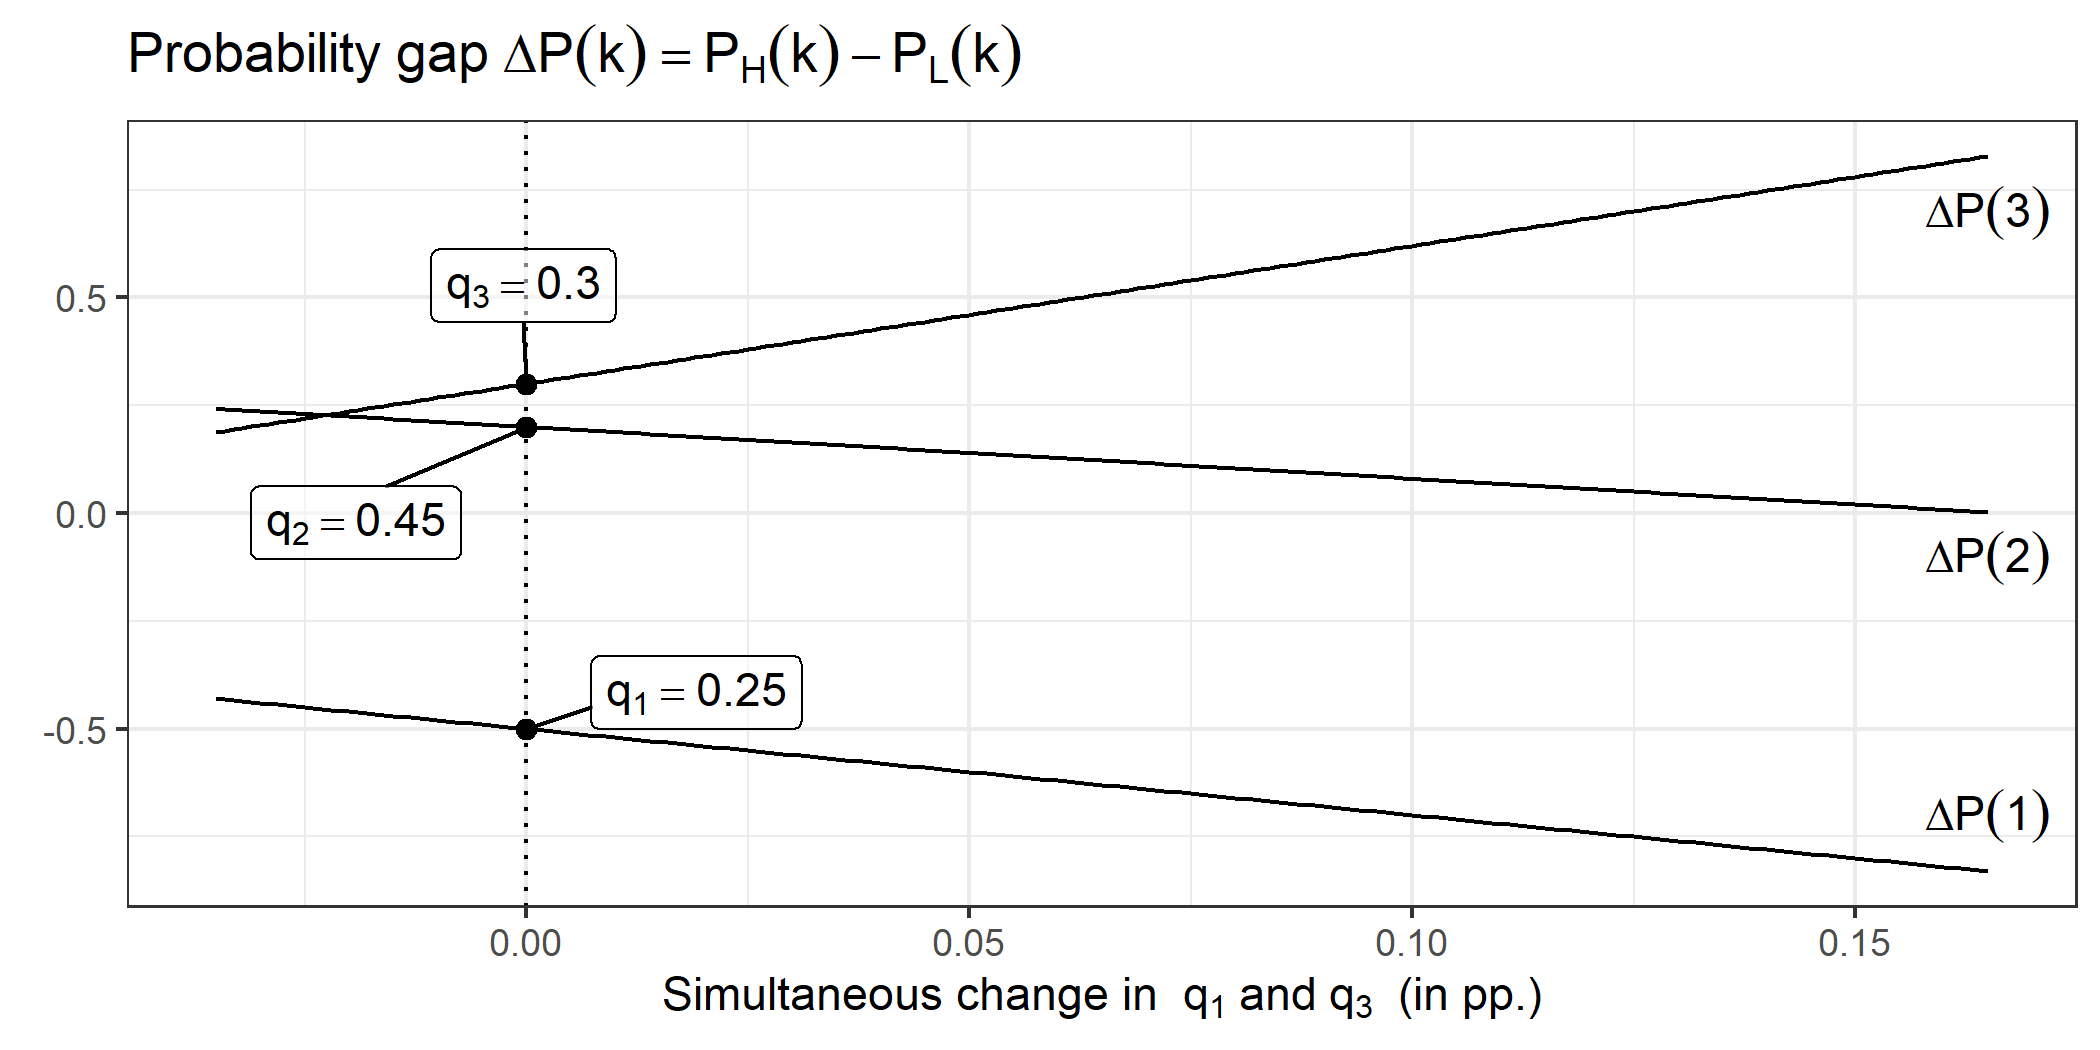
\includegraphics[width=\linewidth]{chap2/graphic/theory-proba-gap.png}
	\vspace{-3em}
	\justify\singlespacing\footnotesize{\textit{Notes:} This figure presents the probability gap in second-period occupations between children from $H$ and $L$ parental income, i.e. $\Delta P(k)$, according to changes in the share of low- and high-paying jobs, i.e. $q_1$ and $q_3$.
	Changes in $q_1$ and $q_3$ are of equal magnitude and at the expense of $q_2$ since $q_1+q_2+q_3=1$.
	Parameters of the model are set such that $z_L = 0.5$, $z_H = 0.5$, and $\pi = 0.25$. The dotted line represents the baseline occupational distribution where $q_1=0.3$, $q_2=0.45$, and $q_3=0.25$.}
\end{figure}
The initial distribution of occupations is assumed to be such that 25\% of workers are in low-paying, 45\% in middling, and 30\% in high-paying occupations. These are figures close to those found in the data, as we will see below. To capture polarization we increase simultaneously $q_{1}$ and $q_{3}$ by the same amount, reducing $q_2$ until only 15\% of workers are in middling occupations (and 40\% and 45\% in $q_1$ and $ q_3$ respectively). The horizontal axis depicts the change in $q_{1}$ and $q_{3}$ in percentage points.

The figure indicates that as polarization increases the advantage in accessing high-paying occupation that those from high-income background have relative to those from low-income households rises. The opposite occurs with low-paying occupations, where the relative likelihood of being in such jobs (which is negative, as only $L$-workers are employed in occupation 1) grows in absolute value with polarization. $H$-workers also have an advantage in being in occupation 2 for low level of polarization, but this advantage falls as $q_1$ and $q_3$ increase, and for high levels of polarization there are more $L$-workers than $H$-workers in middling jobs. The reason for this is that as $q_1$ increases, fewer high-ability $L$-workers manage to move to high-paying occupations, raising their likelihood to be in middling occupations and increasing the number of high-paying jobs available for low-ability $H$-workers. \footnote{In the Appendix we examine separately the effect of changes in $q_1$ and $q_3$ and show that an increase in either of them tends to raise the probability gap between the two types of workers.}

Our results imply a negative relationship between the extent of polarization and the degree of occupation mobility. Greater employment polarization---as measured by an increase in $q_{1}$ and $q_{3}$---reduces mobility by making the distribution of occupations of mature workers more dependent on parental background. This relationship could exist both over time or across locations. If two cohorts of workers face different degrees of polarization when they enter the labour market, we expect to find a lower degree of mobility for the one that experienced a lower share of middling jobs. Similarly, when comparing workers in two geographical areas, we expect to find lower mobility for those based in the location where polarization is greatest.